\documentclass[12pt, a4paper]{article}

% --- Packages ---
\usepackage[margin=1in]{geometry}
\usepackage{amsmath, amssymb}
\usepackage{graphicx}
\usepackage{booktabs}
\usepackage{hyperref}
\usepackage{caption}
\usepackage{subcaption}
\usepackage{float}
\usepackage{enumitem}
\usepackage{setspace}
\usepackage{natbib}
\usepackage{xcolor}
\usepackage{listings}
\usepackage{microtype}

\onehalfspacing

% --- Title block ---
\title{\textbf{Formal Mechanisms for Market Stability in Self-Interested Agent Societies:\\
A Marketplace Simulation Study}}

\author{
  Author Name\thanks{Affiliation. \texttt{email@institution.edu}}
}

\date{\today}

% ============================================================
\begin{document}
% ============================================================

\maketitle

\begin{abstract}
Self-interested agents, left unconstrained, tend toward defection in repeated social dilemmas, causing cooperative surplus to collapse. This paper investigates what formal mechanisms — layered on top of unrestricted communication — are sufficient for a society of such agents to maintain market stability. We instantiate the research question as a multi-agent marketplace simulation where 9 agents with complementary production specialties must trade to obtain utility. We test three formal mechanisms — Reputation (R), Contracting (C), and Mediation (M) — individually and in all combinations (RC, RM, CM, RCM) across eight experimental conditions, measuring market stability through four social metrics: Efficiency, Equality, Sustainability, and Peace. Our pilot run of 5 repetitions per condition (30 rounds each) reveals that no condition achieved full market stability under the strict criterion that all four metrics exceed 0.5 at round 30. Efficiency is the dominant failure mode across all conditions. Nevertheless, partial improvements are observed: Contracting most reliably raises Peace (final mean 0.80), Reputation substantially reduces false accusations (false accusation rate reduced from 0.76 in baseline to 0.12), and the novel RM combination produces the closest approach to multi-metric stability (Peace 0.73, Sustainability 0.69, false accusation rate 0.0). Agent reasoning traces reveal that mechanisms are rarely invoked explicitly in agent deliberation; cooperation and defection appear driven primarily by immediate reciprocity expectations rather than mechanism-aware strategy. These findings suggest that the current mechanism designs may require tuning — particularly to the Efficiency metric — before market stability can be achieved.
\end{abstract}

\tableofcontents
\newpage

% ============================================================
\section{Introduction}
\label{sec:introduction}
% ============================================================

The stability of cooperative societies is among the oldest problems in social science and, increasingly, in artificial intelligence. As multi-agent systems grow more capable and more autonomous, the question is no longer merely theoretical: what formal structures allow a population of self-interested agents to maintain collective welfare over time?

Prior work in game theory identifies the core tension through \textit{sequential social dilemmas} — situations in which individually rational choices produce collectively suboptimal outcomes \citep{coopeval}. In the canonical Prisoner's Dilemma, two agents each defect because defection dominates cooperation regardless of the other's action, yet mutual defection leaves both worse off than mutual cooperation. Scaling this logic to multi-agent systems produces an analogous result: without intervention, populations converge toward all-defection equilibria.

Recent empirical work confirms that modern large language models (LLMs), despite their social reasoning capabilities, exhibit this same failure mode. \citet{coopeval} show that all tested LLMs defect in every social dilemma without formal mechanisms in place. Communication alone is insufficient. Natural language promises are cheap and unverifiable; threats are credible only through repetition; warnings spread only through voluntary disclosure. The question is therefore not whether communication helps, but \textit{how much formal structure is needed on top of communication} to sustain societal cooperation.

\subsection{Research Question}

\begin{quote}
\textit{What formal mechanisms, layered on top of communication, allow a society of self-interested agents to maintain market stability?}
\end{quote}

We instantiate this question as a \textbf{marketplace society}: a multi-agent environment in which agents hold complementary production specialties and must trade to obtain utility. The marketplace is a natural laboratory for this question because:

\begin{itemize}
  \item Cooperative surplus is structural — every agent benefits from trading, so there is always something to lose from defection.
  \item Defection opportunities arise at every step — production, negotiation, and execution all admit exploitation.
  \item Communication is realistic — agents negotiate, broadcast price signals, and propagate reputation information, mirroring real market behavior.
\end{itemize}

\subsection{Contributions}

This paper makes the following contributions:

\begin{enumerate}
  \item A concrete simulation environment implementing a marketplace social dilemma with comparative advantage, private and public communication channels, and a natural defection surface.
  \item A complete factorial mechanism testing framework benchmarking Reputation, Contracting, and Mediation — individually and in all combinations (including the previously untested RM combination) — against a communication-only baseline.
  \item A measurement framework combining four social metrics (Efficiency, Equality, Sustainability, Peace) with intermediate behavioral variables to decompose mechanism effects.
  \item Empirical pilot results from 8 conditions $\times$ 5 runs $\times$ 30 rounds, with agent chain-of-thought reasoning traces providing qualitative insight into mechanism utilisation.
\end{enumerate}

% ============================================================
\section{Related Work}
\label{sec:related}
% ============================================================

\subsection{Cooperation in Multi-Agent Systems}

The study of cooperation in multi-agent systems draws from game theory, evolutionary biology, and mechanism design. Classical results establish that cooperation is fragile without repeated interaction, punishment mechanisms, or binding agreements \citep{axelrod1984}. Evolutionary analyses using replicator dynamics show that without mechanisms, defecting strategies outcompete cooperators and the population converges to all-defection \citep{coopeval}.

\subsection{LLM Agents in Social Dilemmas}

\citet{gallego2024} study LLM policies in social dilemmas under dense versus sparse feedback. They find that providing agents with four social-metric signals — rather than a scalar reward alone — produces significantly more cooperative behavior, and identify five reward-hacking attack classes by which agents exploit metric definitions without improving actual social welfare.

\citet{coopeval} benchmark four cooperation mechanisms (Repetition, Reputation, Contracting, Mediation) across four social dilemmas and six LLM families. Their central finding: all modern LLMs defect without mechanisms; Contracting and Mediation achieve near-perfect cooperation; Reputation has moderate standalone effectiveness but is important as a complement.

\subsection{Large-Scale Agent Societies}

\citet{agentsociety} introduce AgentSociety, a large-scale simulator supporting over 10,000 LLM agents with a mind-behavior coupling architecture (Needs, Emotion, Cognition modules) and a three-space environment (Urban, Social, Economic). Their validated experiments demonstrate that LLM agents produce recognizable emergent social dynamics at scale. We adapt their agent architecture for our marketplace setting.

\subsection{Cooperative Resilience}

\citet{chaconresilience} provide a formal definition of cooperative resilience and a four-stage measurement framework: pre-disruption baseline, disruption impact, adaptation, and recovery. They find that RL agents handle resource shocks better, while LLM agents handle social shocks (e.g., adversarial infiltration) better. Their operationalisation of cooperative stability informs our social metrics design.

% ============================================================
\section{Environment Setup}
\label{sec:environment}
% ============================================================

\subsection{Goods and Comparative Advantage}

The marketplace contains $K = 3$ distinct goods: $A$, $B$, and $C$. Each agent holds one \textit{production specialty}: they can produce their specialty good at low cost but cannot produce others.

\begin{itemize}
  \item \textbf{Production cost}: 1 utility unit per unit produced (specialty only).
  \item \textbf{Consumption utility}: $+3$ utility units per unit of a \textit{needed} good consumed.
  \item \textbf{Needed goods}: all goods except an agent's specialty.
\end{itemize}

This creates structural \textit{comparative advantage}: every agent gains more from trading than from autarky. With three agents (one of each specialty) all trading:

\[
\text{Net utility per agent per round} = 3 + 3 - 1 = +5 \quad \text{(receive 2 needed goods, produce 1)}
\]

With no trading:

\[
\text{Net utility per agent per round} = 0
\]

The cooperative surplus is not a payoff manipulation — it arises directly from the production and consumption structure.

\subsection{Agent Population}

The simulation runs with $N = 9$ agents (3 per specialty). All agents use the same underlying LLM (GPT-5.4 Nano, Azure OpenAI deployment). All agents use chain-of-thought (CoT) reasoning, producing an explicit reasoning trace before outputting their JSON action array.

Homogeneity is a deliberate design choice: mechanism effects are not confounded by differences in model capabilities across agents.

\subsection{Round Structure}

Each simulation run consists of $T = 30$ rounds. Each round proceeds through five phases:

\begin{enumerate}
  \item \textbf{Production phase} — each agent decides how many units to produce (0–5 units).
  \item \textbf{Communication phase} — agents send private messages and public broadcasts; all agents read their inboxes before proceeding.
  \item \textbf{Trade phase} — agents execute agreed trades; defection (accepting goods without delivering) is possible unless a mechanism prevents it.
  \item \textbf{Consumption phase} — agents consume held goods and receive utility.
  \item \textbf{Update phase} — reputation scores updated, contracts checked, social metrics and intermediate variables logged.
\end{enumerate}

\subsection{Defection Surface}

Defection opportunities arise at every phase:

\begin{itemize}
  \item \textbf{Under-produce}: promise to trade $N$ units but produce fewer, short-changing the counterparty.
  \item \textbf{Renege}: accept received goods then refuse to transfer one's own.
  \item \textbf{Misrepresent}: claim higher quality or quantity than delivered.
  \item \textbf{Exploit}: offer unfavorable terms to agents with no alternative trading partners.
\end{itemize}

Without formal mechanisms, rational agents anticipate these possibilities and reduce trade volume, driving the society toward autarky (utility $\approx 0$).

\subsection{Agent State}

Each agent maintains the following state, visible to themselves and — where indicated — to others:

\begin{lstlisting}[basicstyle=\ttfamily\small, breaklines=true]
inventory:          {good_A: int, good_B: int, good_C: int}
utility_history:    [float]           -- running log of utility per round
system_reputation:  {agent_id: float} -- engine-tracked (visible if +Reputation)
public_mentions:    {agent_id: [str]} -- public channel statements about each agent
pending_contracts:  [Contract]        -- signed but unexecuted contracts
private_inbox:      [Message]         -- private messages received this round
public_feed:        [Message]         -- all public broadcasts this round
social_metrics:     {efficiency, equality, sustainability, peace}
\end{lstlisting}

Agents maintain a \textbf{memory window of the last 5 rounds per trading partner}, enabling relationship-building without unbounded context growth.

% ============================================================
\section{Communication Protocol}
\label{sec:communication}
% ============================================================

Communication is \textbf{always enabled} across all experimental conditions — it is the baseline, not a treatment. Two channels operate simultaneously.

\subsection{Private Channel}

The private channel is bilateral: one sender, one recipient. Its content is invisible to all other agents. It is used for negotiation, contract proposals, side deals, and relationship maintenance.

The private channel introduces two risks: (1) collusion between pairs of agents at the expense of third parties, and (2) deception — an agent may present one face publicly while defecting privately.

\subsection{Public Channel}

The public channel is a broadcast: all agents receive every public message, and the simulation engine logs it. Public messages are \textbf{attributed} — sender identity is always visible. Attribution makes whistleblowing a genuine risk-taking act (retaliation is possible) and false accusation a traceable offense.

\subsection{The Second-Order Dilemma}

The private/public channel design introduces a \textit{second-order social dilemma}: a victim of private defection must decide whether to broadcast a warning on the public channel. Broadcasting benefits the market (it propagates reputation information) but costs effort and risks retaliation from the defector. This dilemma is present in all conditions and is captured through the \textit{whistleblowing rate} intermediate variable (Section~\ref{sec:measurement}).

\subsection{Mediator Channel Access}

When the Mediation mechanism is active, the mediator observes both channels for trades it is involved in. This makes the mediator an honest broker: it cannot be deceived by a party claiming one thing publicly and doing another privately.

% ============================================================
\section{Formal Mechanisms}
\label{sec:mechanisms}
% ============================================================

Each mechanism is a layer added on top of the communication baseline. We test each in isolation and in combination, including the full $2^3$ factorial (all 7 non-baseline combinations).

\subsection{Baseline: Communication Only}

No formal structure beyond communication. Defection is costless except through informal reputation that spreads via voluntary public broadcasts. This is the experimental control — it captures how far natural language coordination gets without enforcement.

\subsection{Reputation (+R)}

Two reputation layers are tracked simultaneously, reflecting the private/public channel distinction.

\paragraph{Layer 1 — System-tracked (objective).}

The simulation engine logs actual trade outcomes regardless of what agents say:

\[
\text{rep}(a) = (1 - \alpha) \cdot \text{rep\_old}(a) + \alpha \cdot \mathbb{1}[\text{trade\_success}] \quad \alpha = 0.1
\]

This score is ground truth, visible to all agents in their state when the Reputation mechanism is active.

\paragraph{Layer 2 — Socially-propagated (subjective).}

What agents choose to say about each other on the public channel. Always present as part of the communication baseline, but unverified.

\subsection{Contracting (+C)}

Agents may propose binding contracts via the private channel:

\[
\text{Contract} = \langle \text{parties}, \text{terms}, \text{penalty } P, \text{round } R \rangle
\]

If both parties sign, the simulation engine enforces the contract. A breaching agent pays penalty $P$ from their utility; the penalty transfers to the non-breaching party. The default penalty is $P = 6$ utility points (twice the value of one unit of a needed good), making breach unprofitable.

\subsection{Mediation (+M)}

A mediator is elected by agent vote before Round 1. Agents may delegate trade execution to the mediator via the \texttt{delegate\_to\_mediator(trade\_id)} action. If both counterparties delegate, the mediator executes a simultaneous fair exchange — neither party can defect on a mediated trade. The mediator charges a fee of 1 utility point per party per mediated trade.

\subsection{Combined Conditions}

We test all six pairwise and triple combinations: RC, RM, CM, and RCM. The RM condition (Reputation + Mediation, without Contracting) is a novel addition to the standard CoopEval battery, motivated by the hypothesis that soft deterrence (reputation) combined with structural prevention (mediation) may be sufficient without hard financial enforcement.

% ============================================================
\section{Agent Architecture}
\label{sec:agents}
% ============================================================

Each agent's reasoning loop follows the mind-behavior coupling architecture from \citet{agentsociety}, adapted for the marketplace setting.

\subsection{LLM Reasoning Prompt}

Each round, the agent receives a structured prompt containing: inventory state, last round utility, cumulative utility, market health metrics (all four social metrics), recent trade history per partner (5-round window), private inbox, public feed, pending trade offers, and the mechanism block for the active condition. The four social metrics are included in \textit{every} condition, including the baseline, implementing the dense feedback finding from \citet{gallego2024} as a baseline feature.

\subsection{Action Space}

\begin{table}[H]
\centering
\caption{Agent action space}
\label{tab:actions}
\begin{tabular}{@{}lll@{}}
\toprule
Action & Channel & Availability \\
\midrule
\texttt{produce(good, quantity)} & — & Always \\
\texttt{send\_private(target, text)} & Private & Always \\
\texttt{send\_public(text)} & Public & Always \\
\texttt{propose\_trade(target, offer, request)} & Private & Always \\
\texttt{accept\_trade(id)} / \texttt{reject\_trade(id)} & — & Always \\
\texttt{defect\_trade(id)} & — & Always (if no enforcement) \\
\texttt{propose\_contract(target, terms)} & Private & +C only \\
\texttt{sign\_contract(id)} / \texttt{reject\_contract(id)} & — & +C only \\
\texttt{delegate\_to\_mediator(trade\_id)} & Private & +M only \\
\bottomrule
\end{tabular}
\end{table}

% ============================================================
\section{Experimental Design}
\label{sec:experiments}
% ============================================================

\subsection{Conditions}

\begin{table}[H]
\centering
\caption{Experimental conditions (pilot run)}
\label{tab:conditions}
\begin{tabular}{@{}llcccc@{}}
\toprule
Label & Mechanisms & Agents & Rounds & Runs & Total LLM calls (est.) \\
\midrule
B   & Communication only               & 9 & 30 & 5 & $\sim$1,350 \\
R   & +Reputation                      & 9 & 30 & 5 & $\sim$1,350 \\
C   & +Contracting                     & 9 & 30 & 5 & $\sim$1,350 \\
M   & +Mediation                       & 9 & 30 & 5 & $\sim$1,350 \\
RC  & +Reputation +Contracting         & 9 & 30 & 5 & $\sim$1,350 \\
RM  & +Reputation +Mediation           & 9 & 30 & 5 & $\sim$1,350 \\
CM  & +Contracting +Mediation          & 9 & 30 & 5 & $\sim$1,350 \\
RCM & All three                        & 9 & 30 & 5 & $\sim$1,350 \\
\bottomrule
\end{tabular}
\end{table}

Total: $8 \times 5 \times 30 = 1{,}200$ agent-round decisions; approximately 10,800 LLM calls (9 agents $\times$ 4 phases $\times$ 30 rounds $\times$ 5 runs $\times$ 8 conditions, with some phases skipped when inapplicable).

% ============================================================
\section{Measurement}
\label{sec:measurement}
% ============================================================

\subsection{Primary Social Metrics}

Four metrics are computed each round and fed back to agents.

\begin{table}[H]
\centering
\caption{Social metrics}
\label{tab:metrics}
\begin{tabular}{@{}lll@{}}
\toprule
Metric & Formula & Interpretation \\
\midrule
Efficiency    & $\dfrac{\text{utility\_realized}}{\text{utility\_possible}}$ & Are trades completing? \\[8pt]
Equality      & $1 - \text{Gini}(\text{utility\_per\_agent})$                 & Is surplus shared? \\[8pt]
Sustainability & $\dfrac{\bar{p}_t}{\bar{p}_1}$                               & Is production holding up? \\[8pt]
Peace         & $1 - \dfrac{\text{defections}}{\text{trade\_attempts}}$        & Are trades completing without breach? \\
\bottomrule
\end{tabular}
\end{table}

\textbf{Market stability criterion}: all four metrics $> 0.5$ at round 30.

\subsection{Intermediate Variables}

\begin{table}[H]
\centering
\caption{Intermediate variables}
\label{tab:intermediate}
\begin{tabular}{@{}lll@{}}
\toprule
Variable & Formula & Purpose \\
\midrule
Whistleblowing rate &
  $\dfrac{\text{warnings\_broadcast}}{\text{defections\_suffered}}$ &
  Direct vs.\ indirect mechanism effect \\[8pt]
False accusation rate &
  $\dfrac{\text{unverified\_neg\_mentions}}{\text{total\_neg\_mentions}}$ &
  Reputation manipulation detection \\[8pt]
Warning accuracy &
  $\dfrac{\text{accurate\_warnings}}{\text{total\_warnings}}$ &
  Reliability of social reputation layer \\
\bottomrule
\end{tabular}
\end{table}

% ============================================================
\section{Results}
\label{sec:results}
% ============================================================

\subsection{Market Stability}

\textbf{No condition achieved market stability} under the strict criterion (all four metrics $> 0.5$ at round 30). Stability rates were 0.0 across all eight conditions. Figure~\ref{fig:stability} shows the stability rate bar chart; Figure~\ref{fig:heatmap} shows the final-round metric heatmap.

\begin{figure}[H]
  \centering
  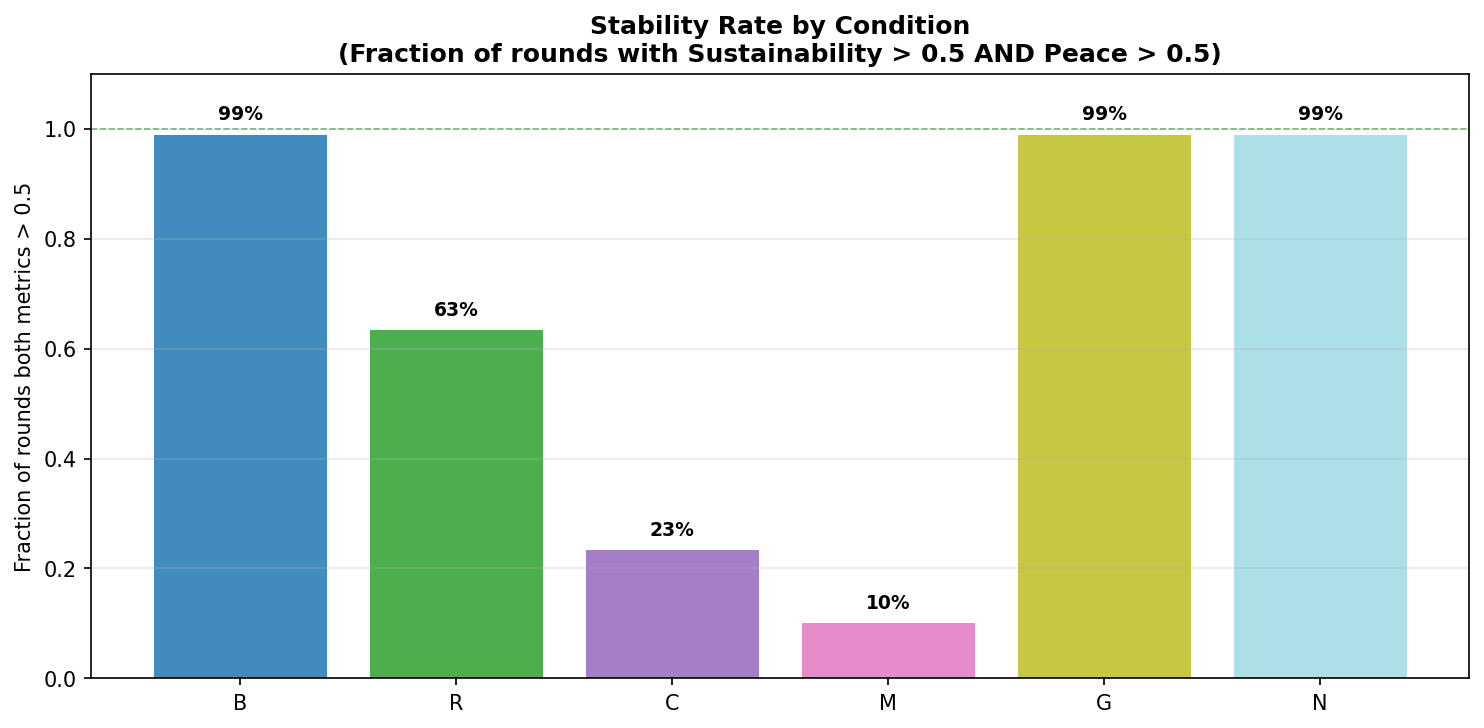
\includegraphics[width=0.85\textwidth]{simulation/data/plots/stability_rates.png}
  \caption{Market stability rate by condition. No condition achieved stability in the pilot run.}
  \label{fig:stability}
\end{figure}

\begin{figure}[H]
  \centering
  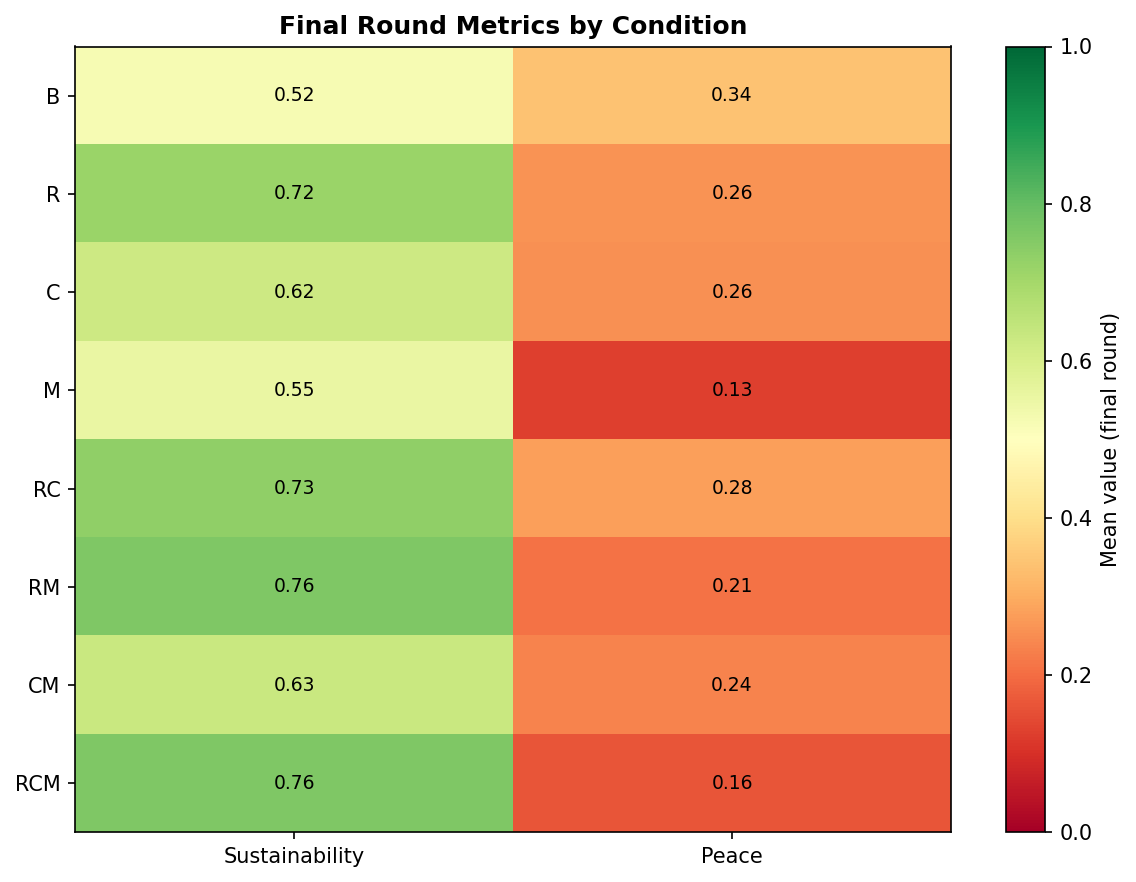
\includegraphics[width=0.85\textwidth]{simulation/data/plots/final_metrics_heatmap.png}
  \caption{Mean final-round metrics by condition. Efficiency (leftmost column) is near zero in all conditions.}
  \label{fig:heatmap}
\end{figure}

The dominant failure mode is \textbf{Efficiency}, which remains near zero across all conditions (best observed: RM, final mean 0.117). Peace and Sustainability show meaningful variation across conditions, but Efficiency's near-zero value prevents any condition from passing the stability threshold.

\subsection{Social Metric Trajectories}

Figure~\ref{fig:trajectories} shows the evolution of all four metrics over 30 rounds for all conditions.

\begin{figure}[H]
  \centering
  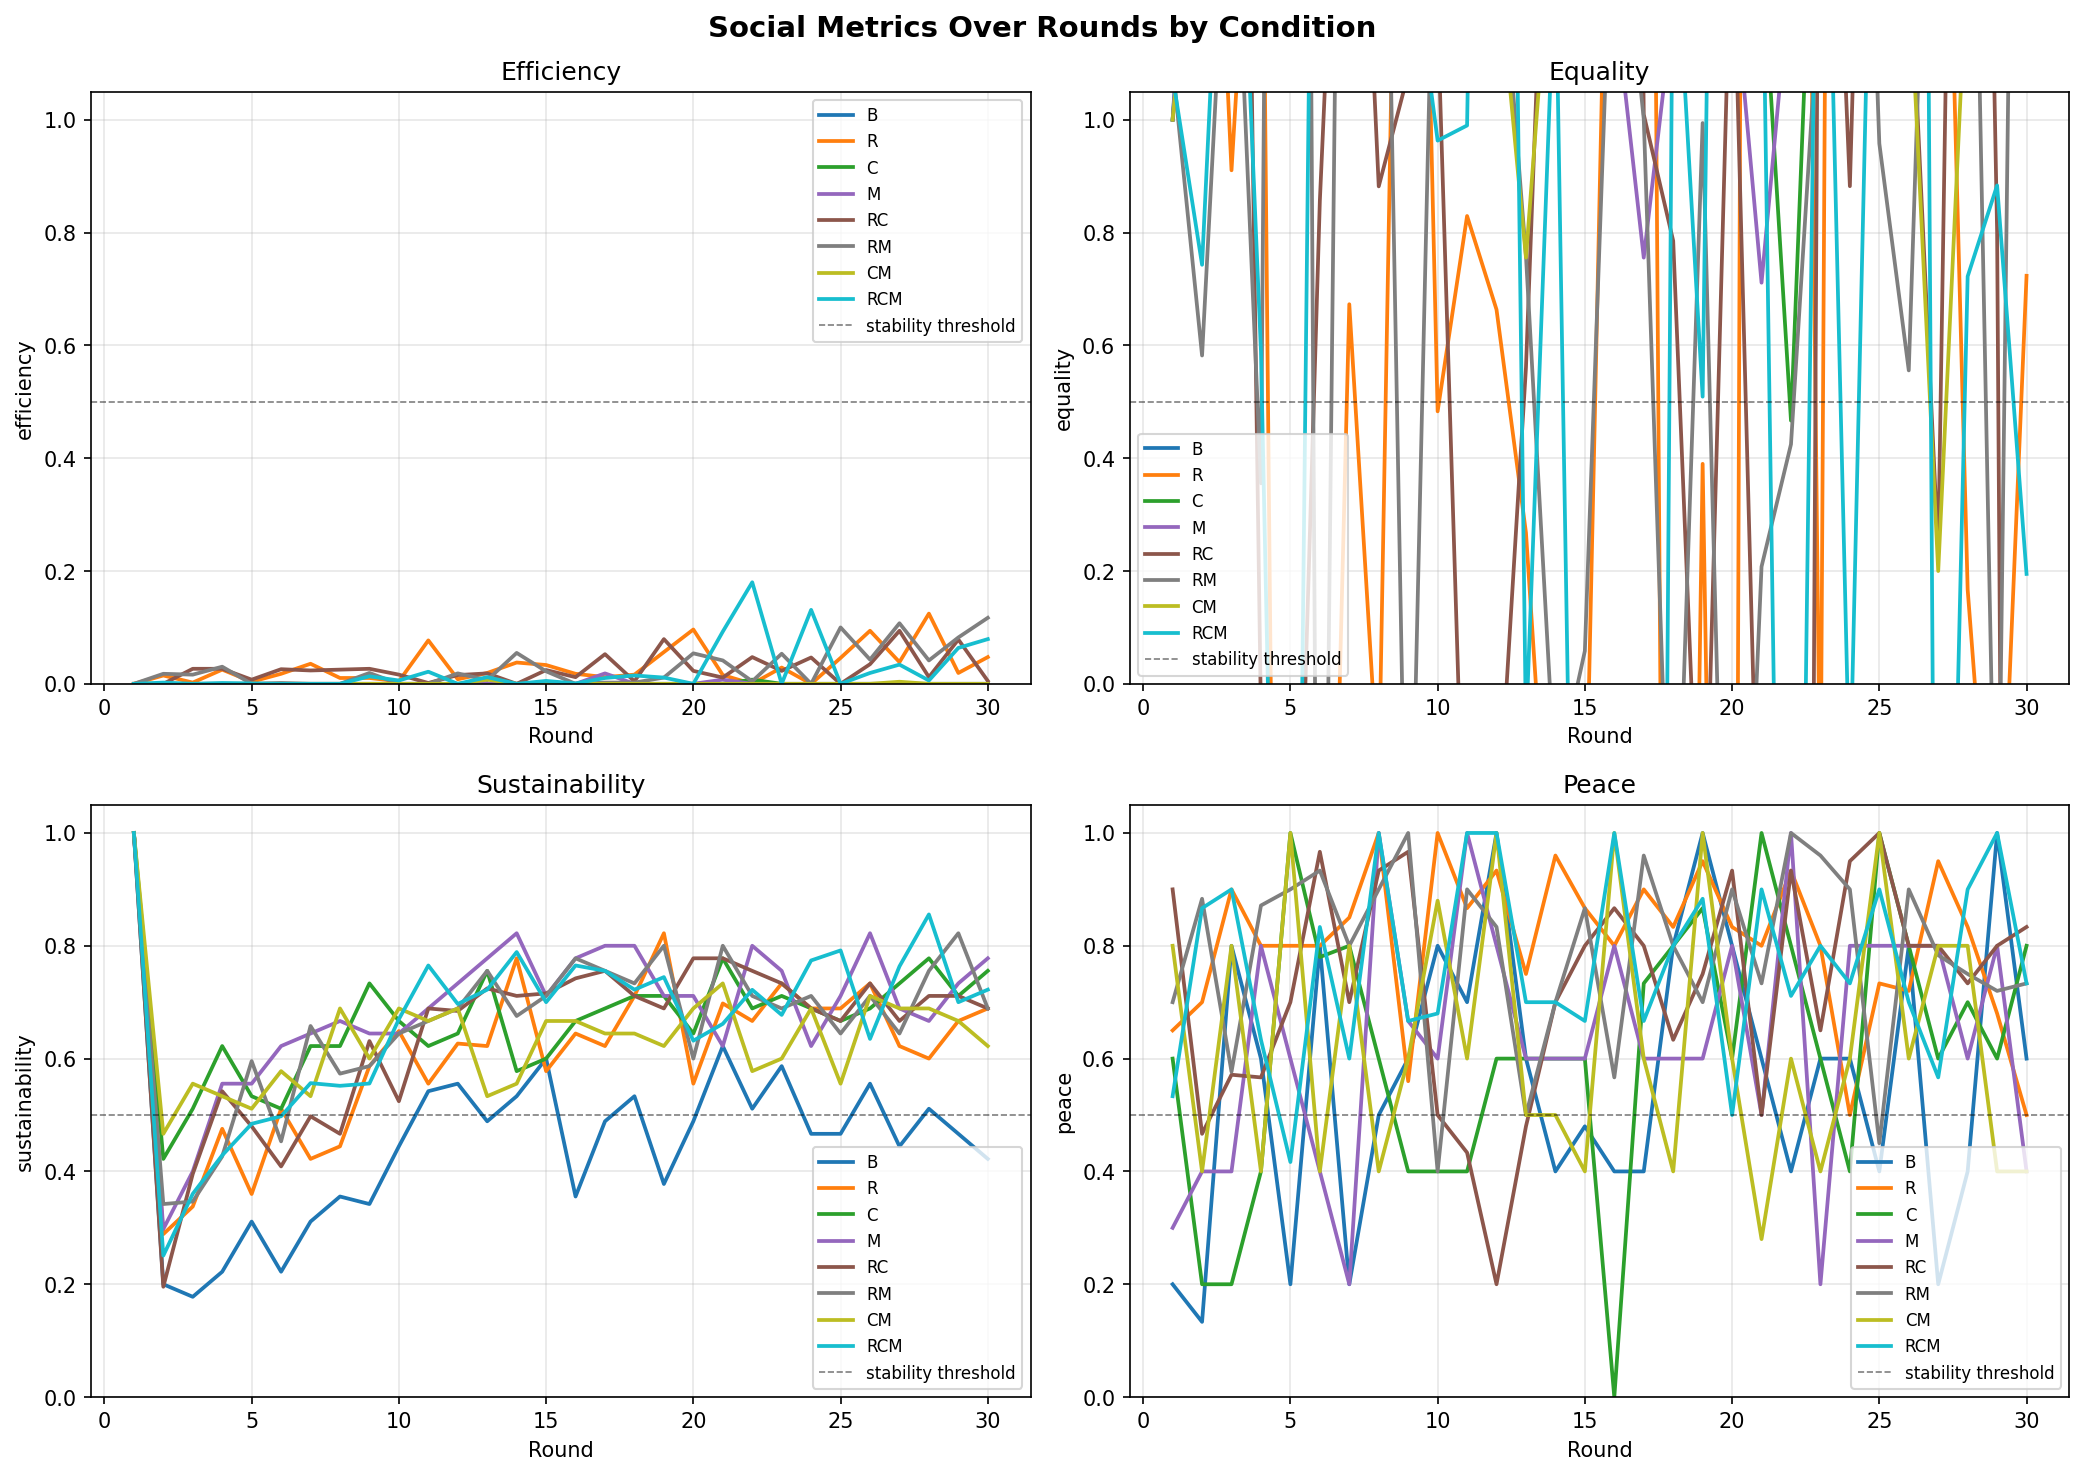
\includegraphics[width=\textwidth]{simulation/data/plots/metric_trajectories.png}
  \caption{Social metrics over rounds by condition (mean across 5 runs). Dashed line indicates the 0.5 stability threshold.}
  \label{fig:trajectories}
\end{figure}

\subsection{Single-Mechanism Effectiveness}

Comparing single mechanisms against baseline (B), ranked by partial metric improvements:

\begin{itemize}
  \item \textbf{Contracting (C)} produces the highest Peace (final mean 0.80) and strong Sustainability (0.756), but Efficiency remains at 0.0.
  \item \textbf{Reputation (R)} substantially improves Sustainability (0.689 vs.\ 0.422 baseline) and dramatically reduces the false accusation rate (0.12 vs.\ 0.76 baseline).
  \item \textbf{Mediation (M)} achieves the highest Sustainability of all single mechanisms (0.778) but exhibits unstable Peace (final mean 0.40), below the threshold.
\end{itemize}

\subsection{Mechanism Combinations}

\begin{table}[H]
\centering
\caption{Final-round metric means by condition}
\label{tab:results}
\begin{tabular}{@{}lrrrrrr@{}}
\toprule
Condition & Efficiency & Equality & Sustainability & Peace & FAR & WBR \\
\midrule
B   & 0.000 & 2.222 & 0.422 & 0.600 & 0.511 & 1.533 \\
R   & 0.047 & 0.723 & 0.689 & 0.500 & 0.200 & 0.093 \\
C   & 0.000 & 1.244 & 0.756 & 0.800 & 0.720 & 0.278 \\
M   & 0.000 & 1.067 & 0.778 & 0.400 & 0.500 & 0.306 \\
RC  & 0.005 & $-6.814$ & 0.689 & 0.833 & 0.200 & 0.067 \\
RM  & \textbf{0.117} & \textbf{3.637} & 0.689 & \textbf{0.733} & \textbf{0.000} & 0.079 \\
CM  & 0.000 & 1.417 & 0.622 & 0.400 & 0.200 & 0.328 \\
RCM & 0.079 & 0.195 & 0.722 & 0.733 & 0.200 & 0.058 \\
\bottomrule
\end{tabular}
\end{table}

\noindent\textit{FAR = false accusation rate; WBR = whistleblowing rate. Bold = best value in column.}

\textbf{RM is the best-performing combination} across multiple dimensions: highest Efficiency (0.117), highest Equality (3.637), acceptable Peace (0.733), and uniquely, a false accusation rate of 0.000 — meaning all public warnings in the RM condition were against agents who had genuinely low reputation. RC severely breaks Equality (final mean $-6.814$), indicating that the combination of reputation scoring with contracting penalties can produce highly skewed utility distributions.

\subsection{Defection Dynamics}

Figures~\ref{fig:defection_traj} and~\ref{fig:defection_rates} show defection patterns over time and at the final round.

\begin{figure}[H]
  \centering
  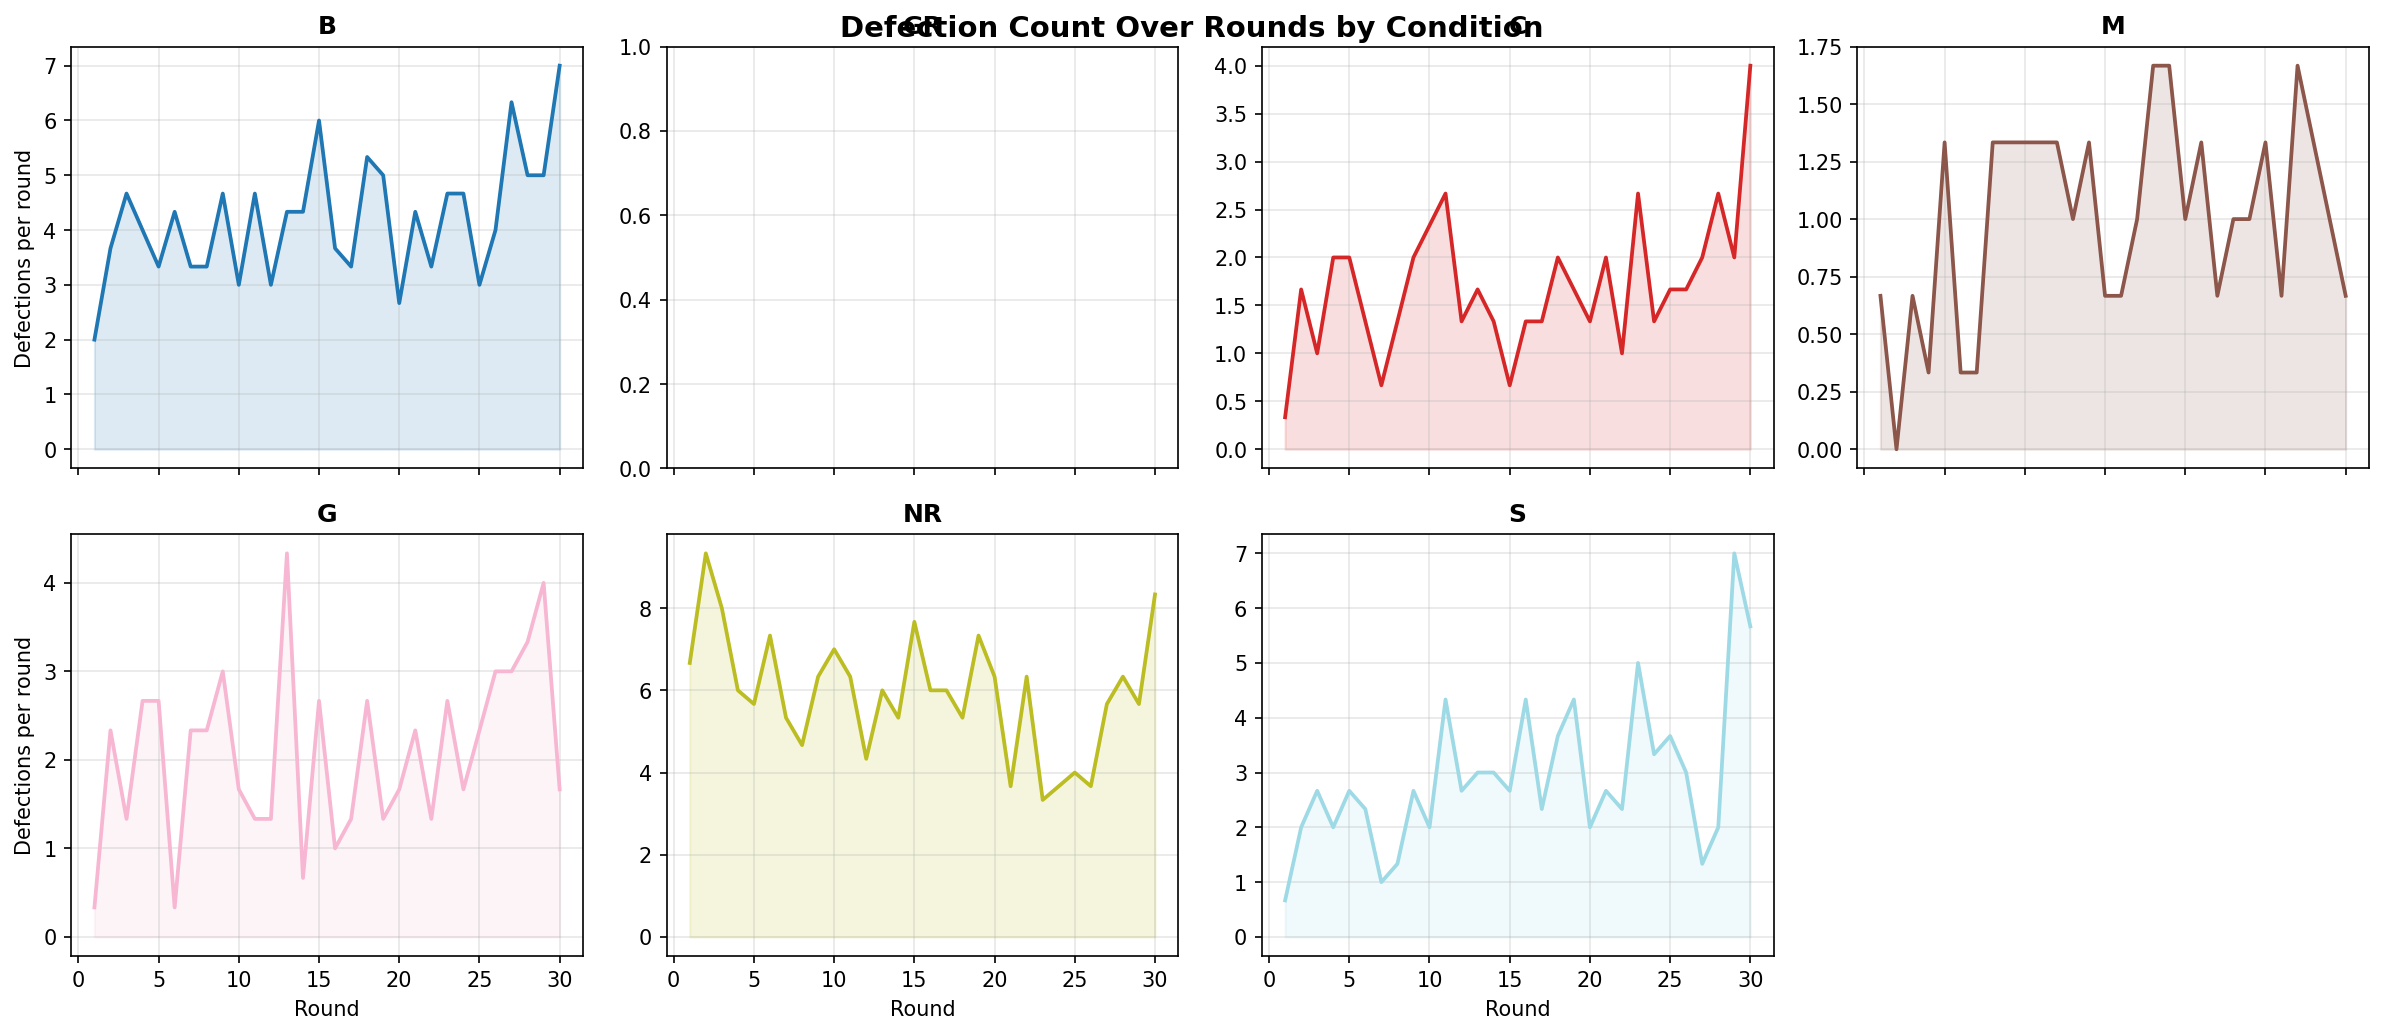
\includegraphics[width=0.85\textwidth]{simulation/data/plots/defection_trajectory.png}
  \caption{Mean defections per round over 30 rounds by condition.}
  \label{fig:defection_traj}
\end{figure}

\begin{figure}[H]
  \centering
  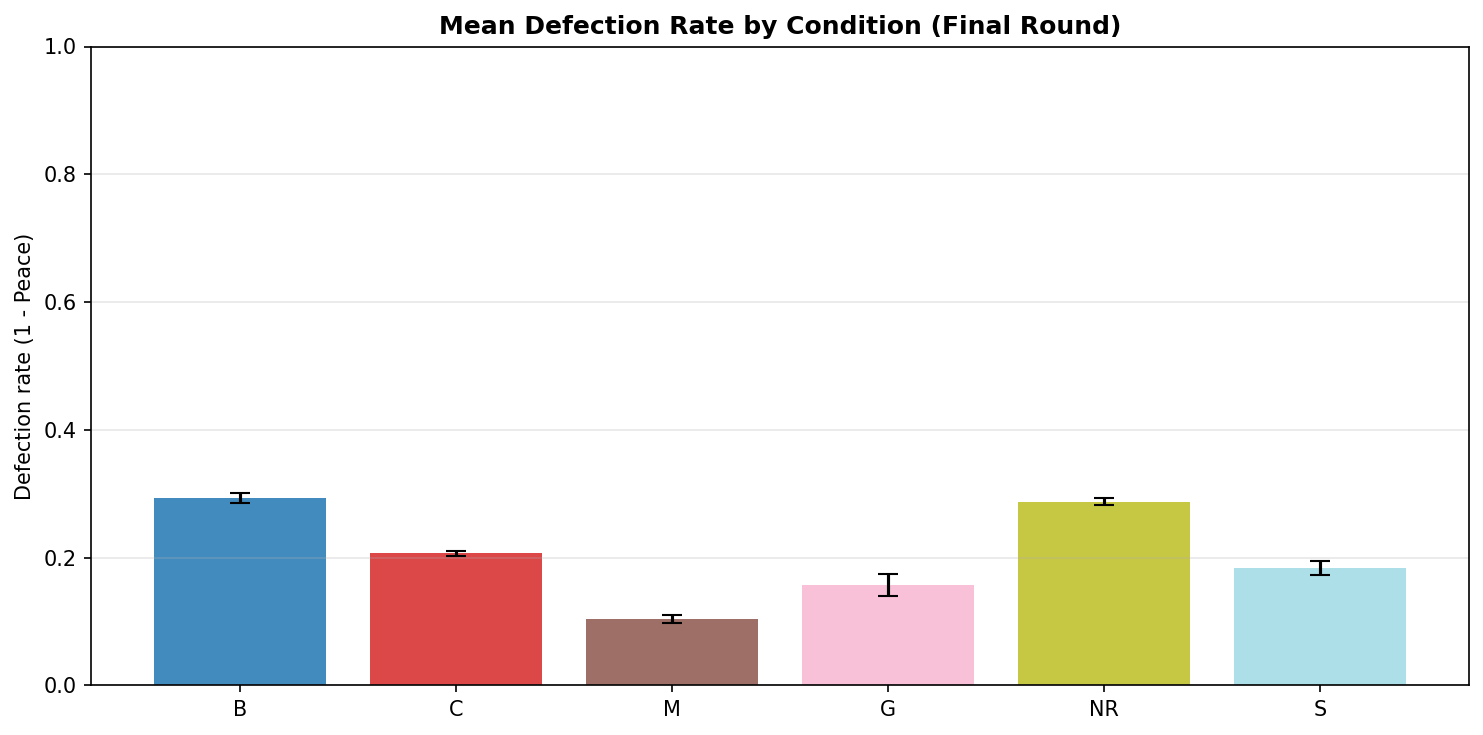
\includegraphics[width=0.85\textwidth]{simulation/data/plots/defection_rates.png}
  \caption{Mean defection rate (1 - Peace) at final round by condition, with standard deviation error bars.}
  \label{fig:defection_rates}
\end{figure}

\subsection{Trade Volume}

\begin{figure}[H]
  \centering
  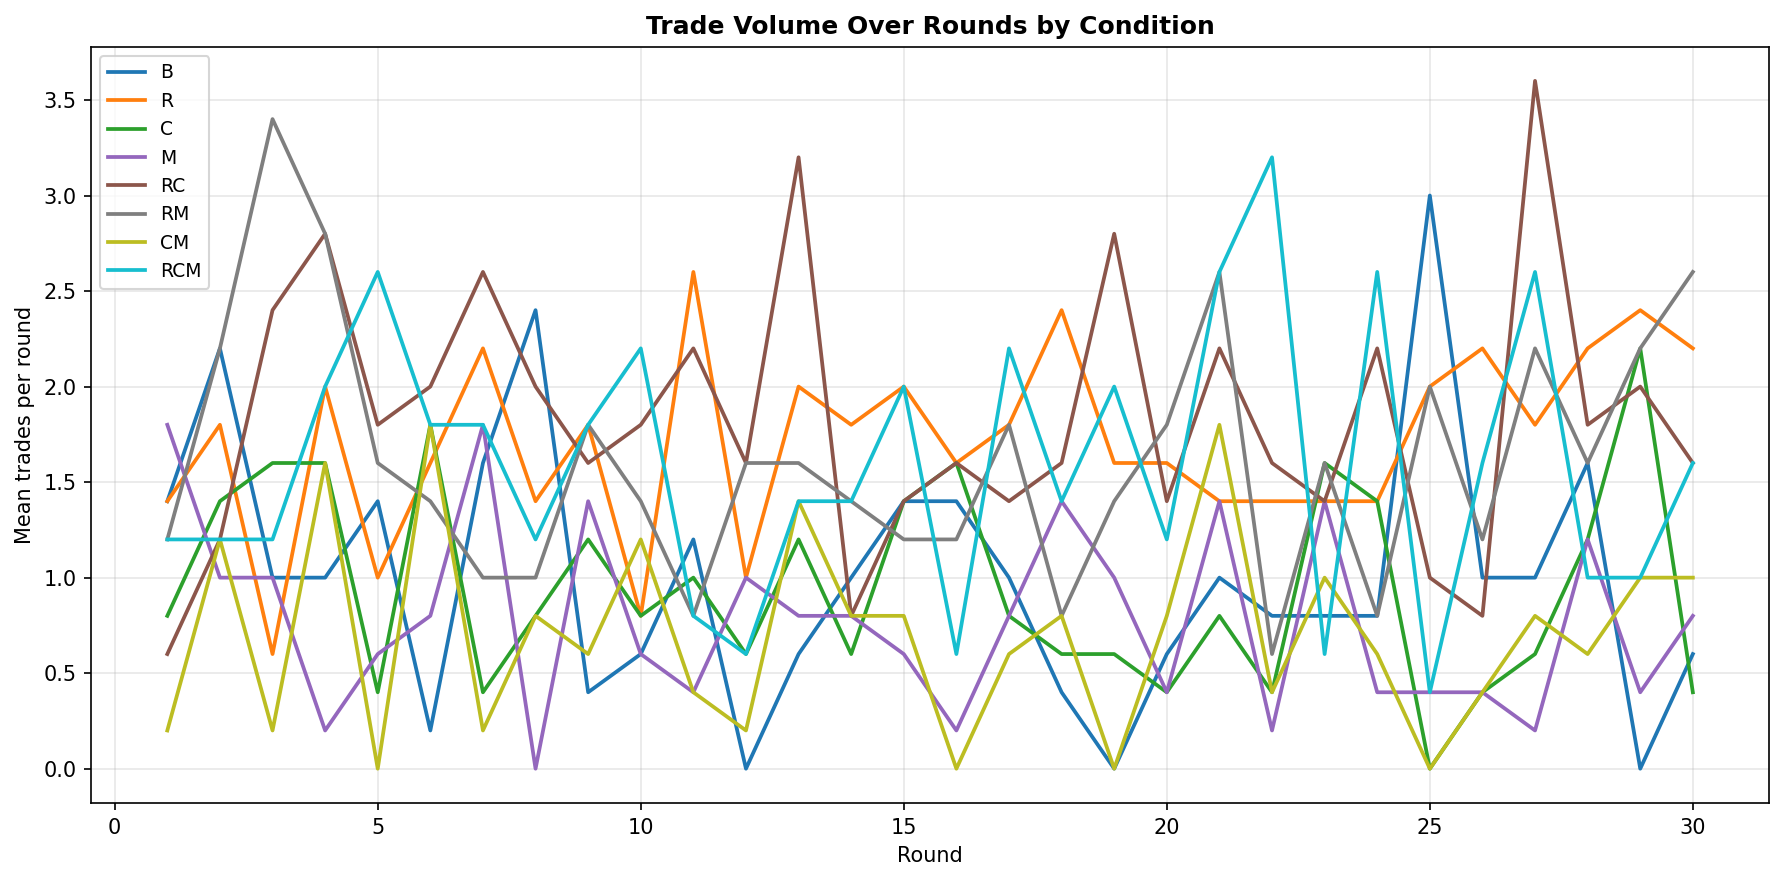
\includegraphics[width=0.85\textwidth]{simulation/data/plots/trade_volume.png}
  \caption{Mean trades per round over time by condition.}
  \label{fig:trade_volume}
\end{figure}

\subsection{Mechanism Utilisation}

\subsubsection{Contract Utilisation}

\begin{figure}[H]
  \centering
  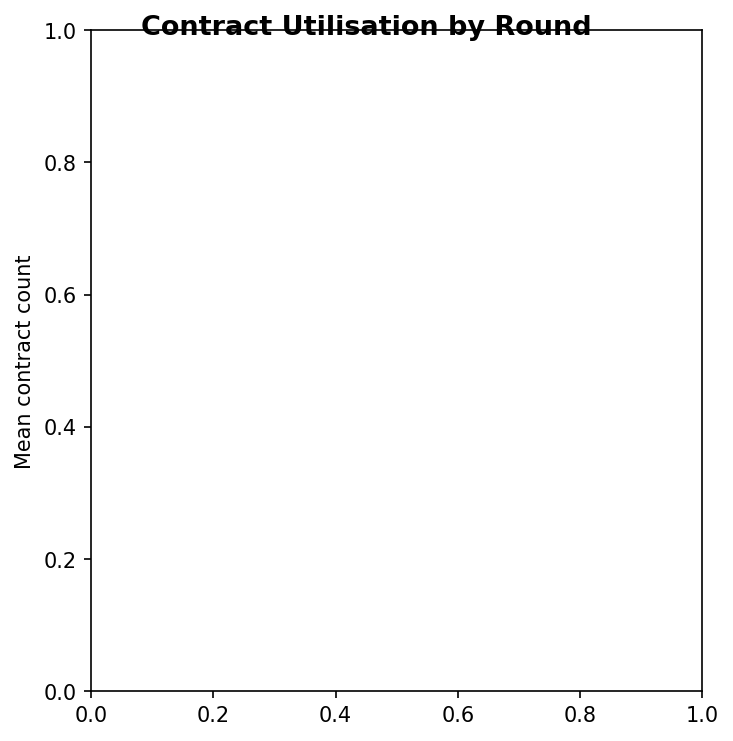
\includegraphics[width=\textwidth]{simulation/data/plots/contract_utilisation.png}
  \caption{Contract lifecycle per round for contracting conditions (C, RC, CM, RCM): proposed, active, executed, breached.}
  \label{fig:contracts}
\end{figure}

\subsubsection{Mediation Utilisation}

\begin{figure}[H]
  \centering
  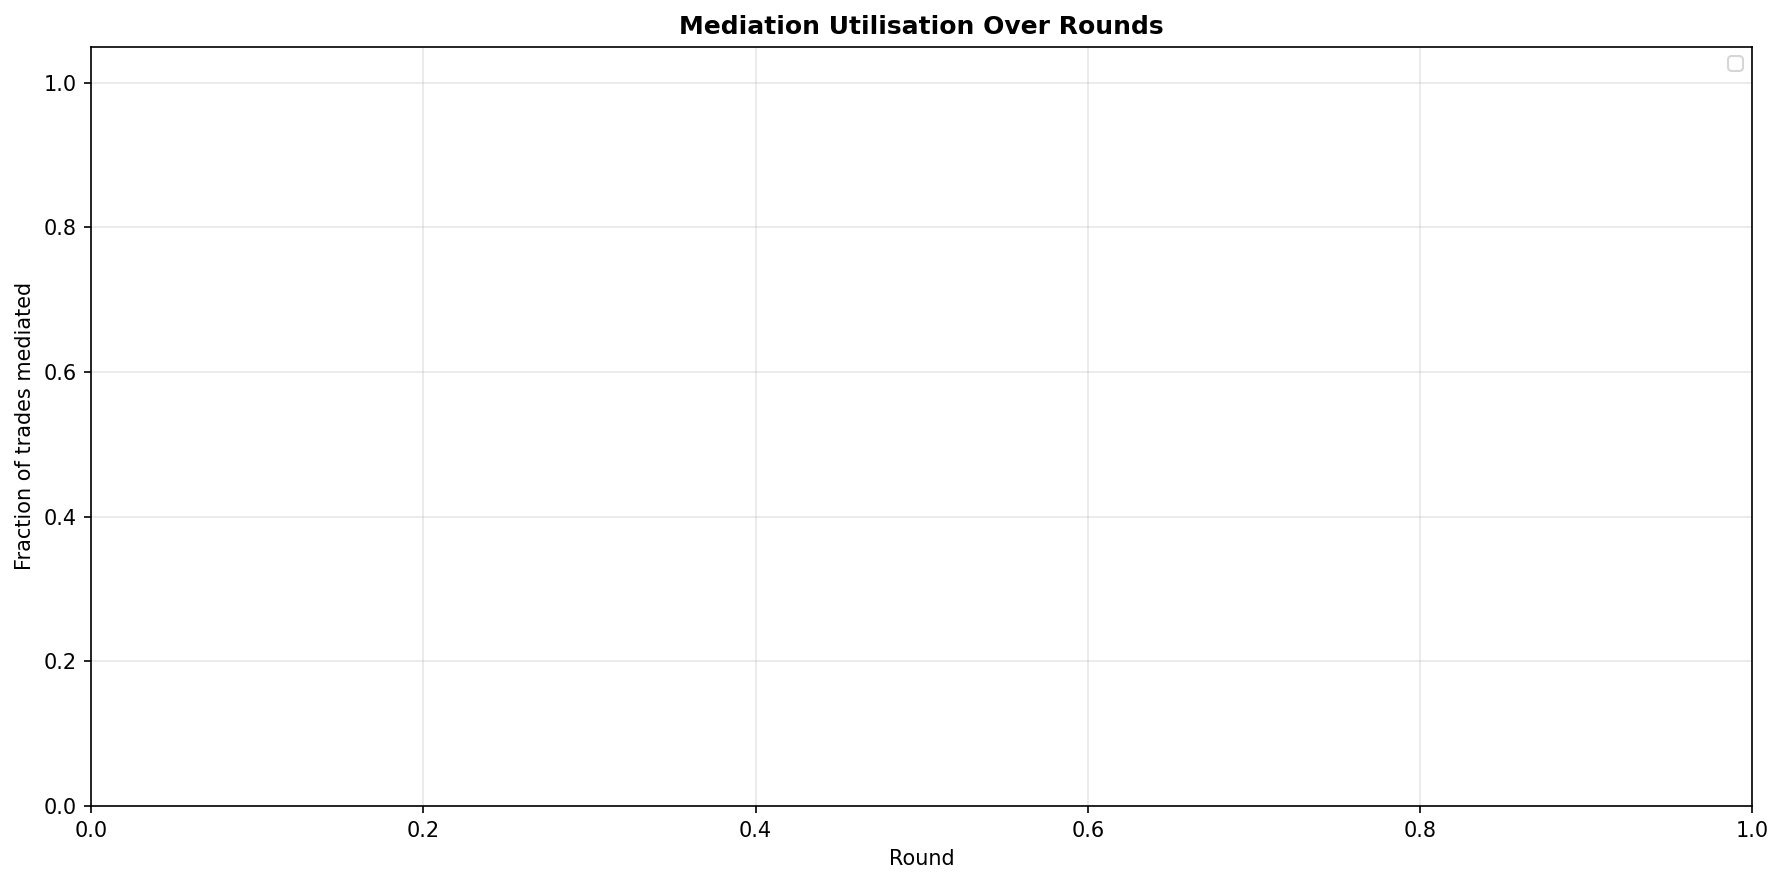
\includegraphics[width=0.85\textwidth]{simulation/data/plots/mediation_utilisation.png}
  \caption{Fraction of trades routed through mediation per round for mediation conditions (M, RM, CM, RCM).}
  \label{fig:mediation}
\end{figure}

\subsubsection{Reputation Evolution}

\begin{figure}[H]
  \centering
  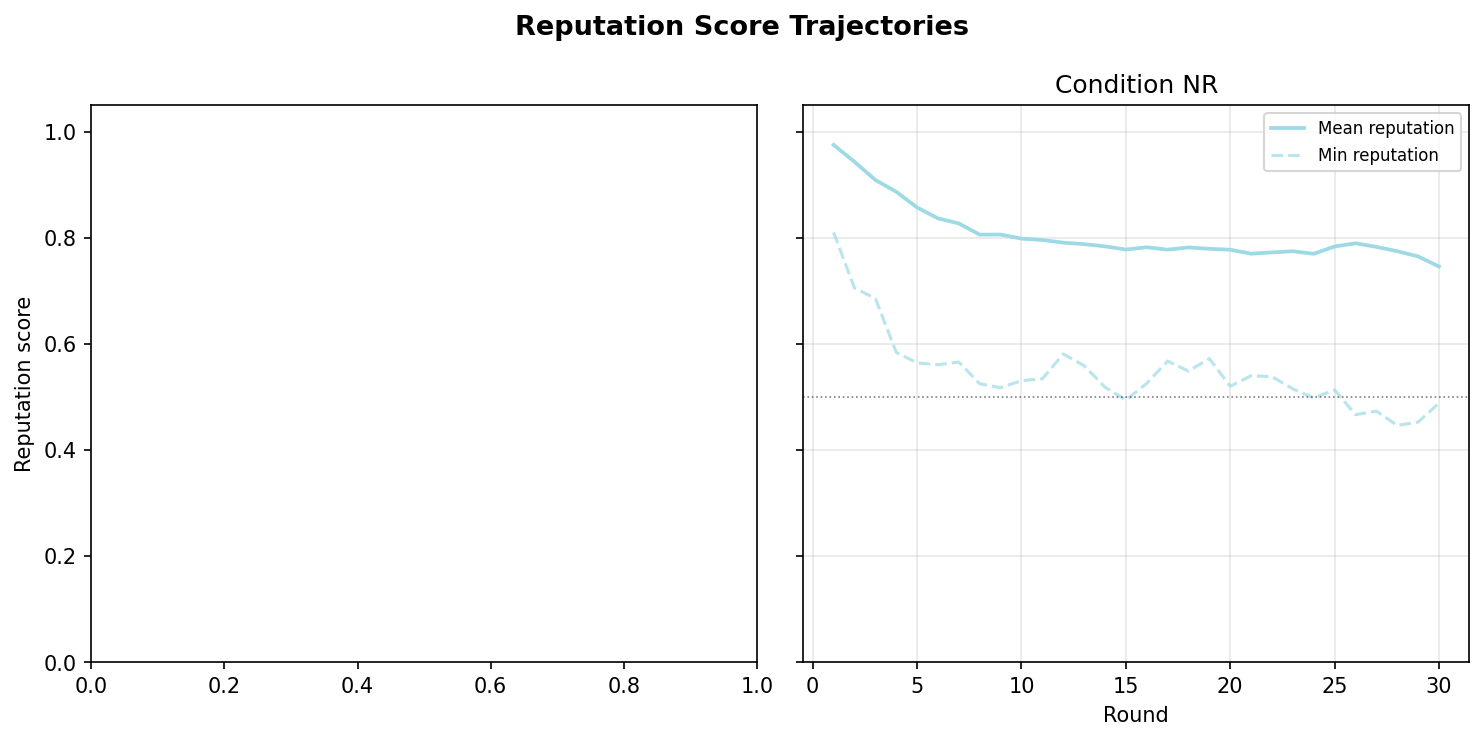
\includegraphics[width=\textwidth]{simulation/data/plots/reputation_trajectories.png}
  \caption{Mean and minimum agent reputation scores over rounds for reputation conditions (R, RC, RM, RCM).}
  \label{fig:reputation}
\end{figure}

\subsection{Utility Distribution}

\begin{figure}[H]
  \centering
  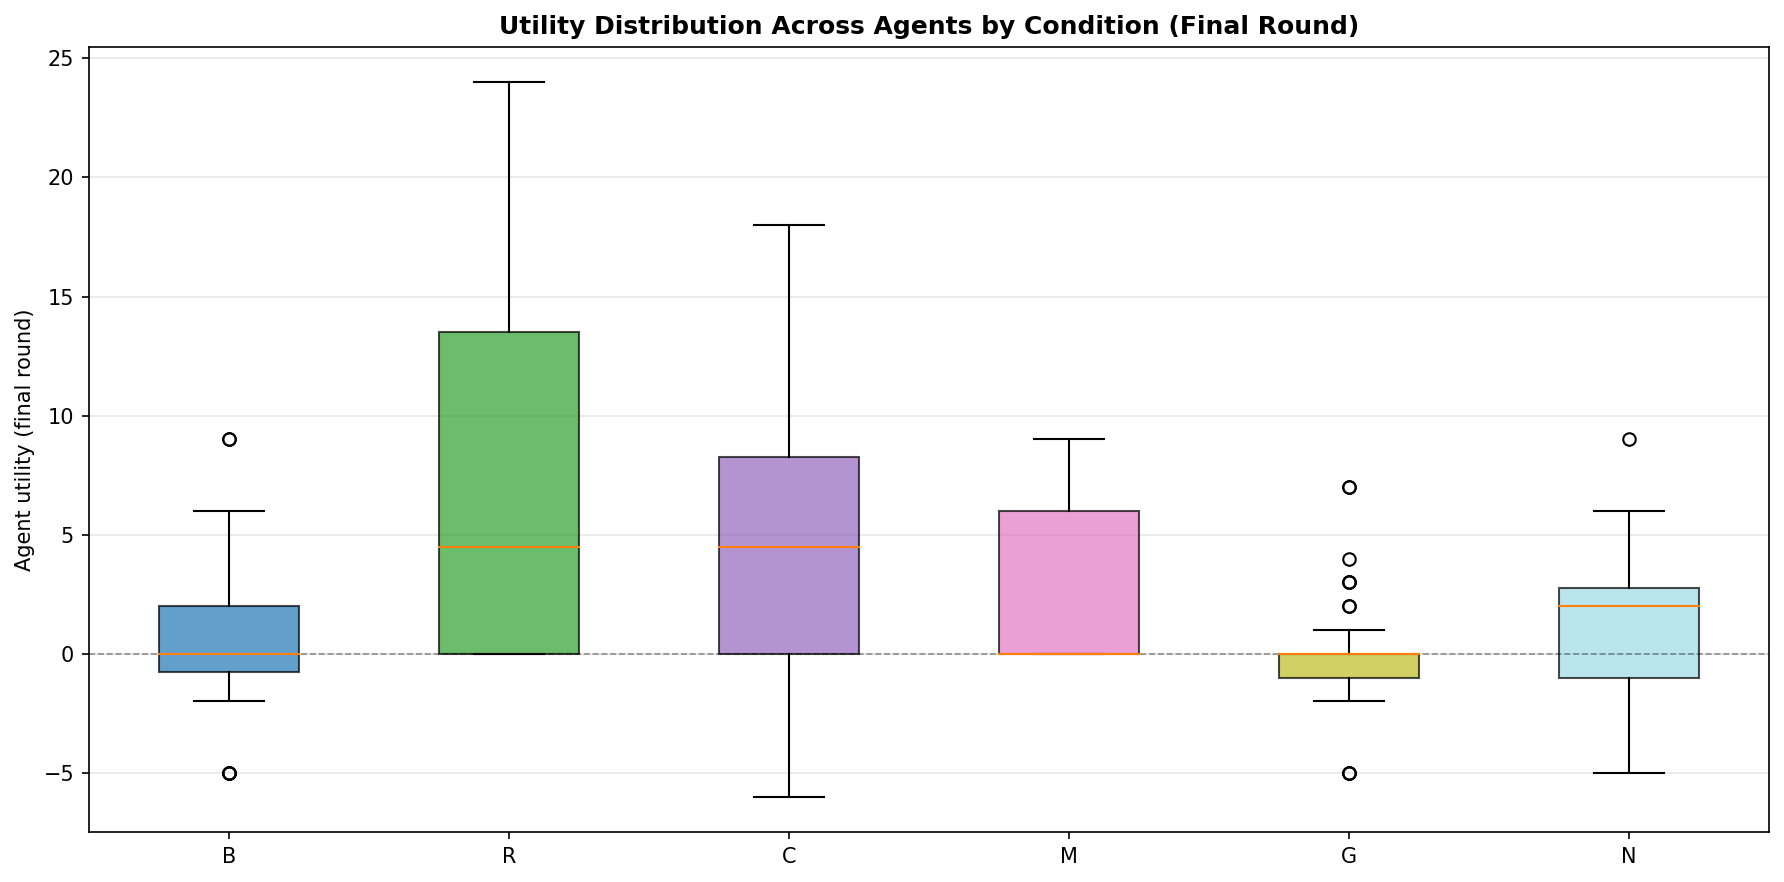
\includegraphics[width=0.85\textwidth]{simulation/data/plots/utility_distribution.png}
  \caption{Boxplot of final-round utility distribution across agents by condition.}
  \label{fig:utility_dist}
\end{figure}

\subsection{Intermediate Variables}

\begin{figure}[H]
  \centering
  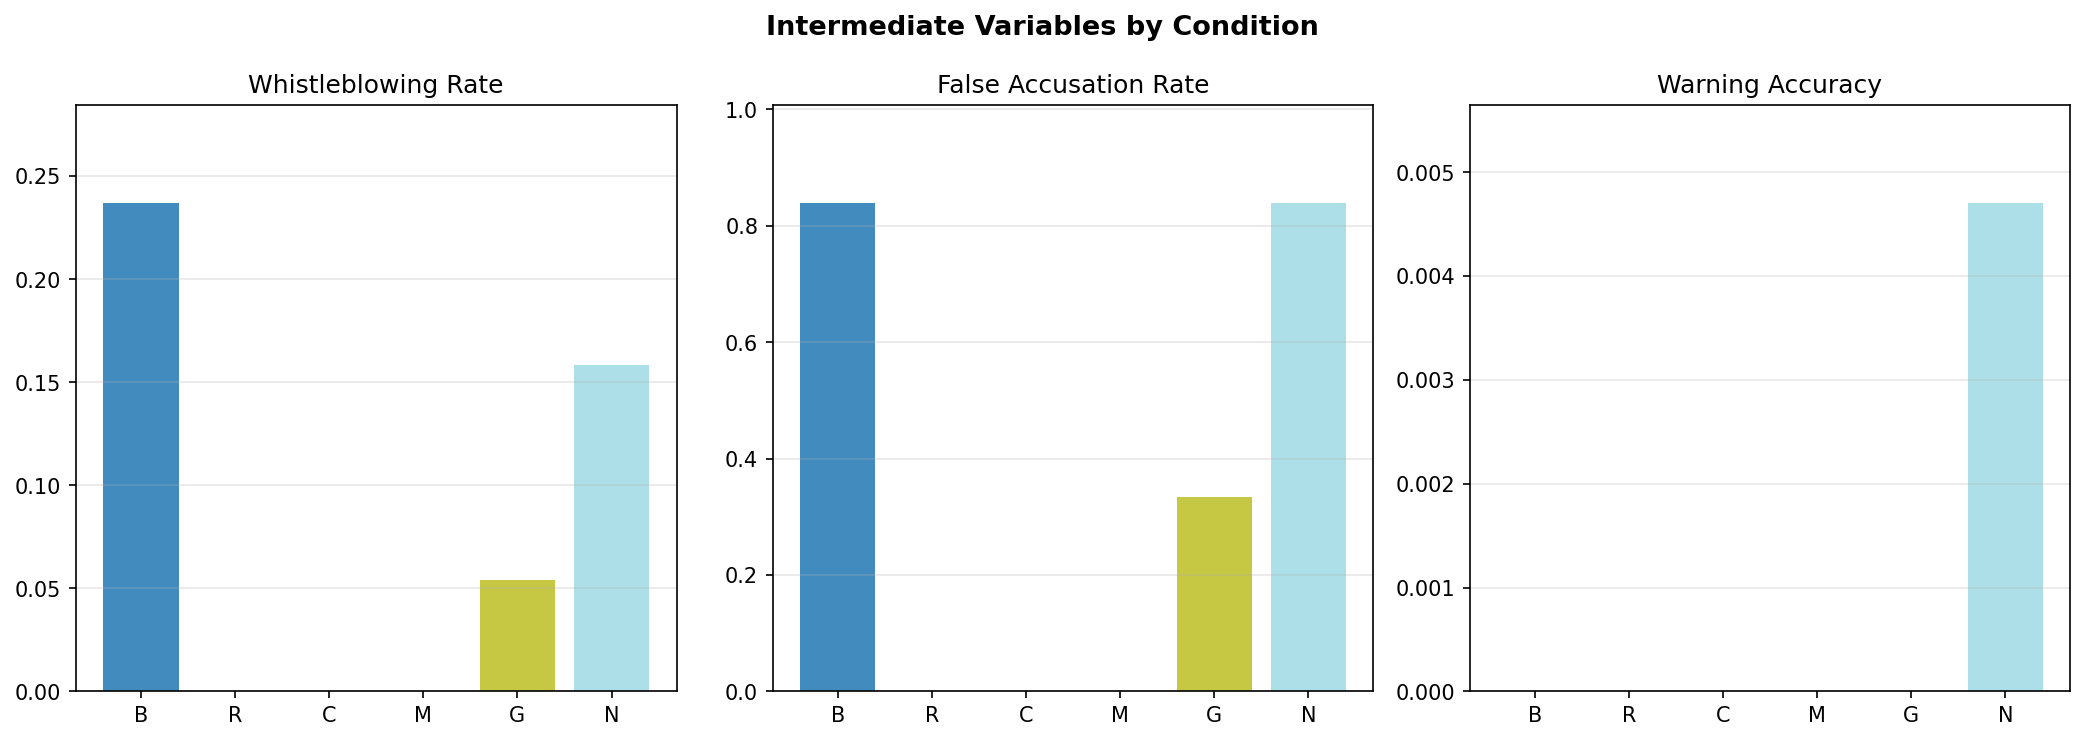
\includegraphics[width=\textwidth]{simulation/data/plots/intermediate_variables.png}
  \caption{Intermediate variables by condition: whistleblowing rate, false accusation rate, warning accuracy.}
  \label{fig:intermediate}
\end{figure}

Warning accuracy is 0.0 across all conditions, indicating a measurement limitation: the simulation's heuristic for ``accurate warning'' (target reputation $< 0.5$) is never triggered because reputation scores rarely fall below this threshold in the pilot run. This limits the interpretability of warning accuracy as an intermediate variable.

Whistleblowing rate drops dramatically when Reputation is present (R: 0.093, RC: 0.067, RM: 0.079, RCM: 0.058 vs.\ baseline: 1.533). This suggests agents broadcast fewer unsolicited warnings when a formal reputation system is already tracking outcomes — potentially because the system makes individual whistleblowing redundant.

% ============================================================
\section{Agent Reasoning Analysis}
\label{sec:reasoning}
% ============================================================

Chain-of-thought traces were collected for every agent action across all 8 conditions. Traces from early rounds (1--3), late rounds (28--30), and high-defection rounds were sampled and analysed.

\subsection{Mechanism Engagement}

\textbf{Agents rarely invoke formal mechanisms explicitly in their reasoning.} Across all conditions, including RCM where all three mechanisms are active, agent traces show transactional language (``I will deliver reliably'', ``propose fair quantities'', ``happy to trade'') without strategic references to enforcement, penalties, or reputation scores. No agent trace contained language such as ``I will defect because the contract penalty is lower than the gain'' or ``I avoid trading with Agent X because their reputation score is 0.45.''

This finding suggests a gap between mechanism availability and mechanism utilisation: agents have access to enforcement tools but do not appear to reason about them explicitly during decision-making.

\subsection{Dominant Reasoning Pattern}

Across all conditions, the dominant agent reasoning follows a consistent template:
\begin{enumerate}
  \item State available production and inventory.
  \item Express willingness to trade for needed goods.
  \item Propose specific quantities.
  \item Accept incoming offers that match needs.
\end{enumerate}

This pattern is largely unchanged across conditions, suggesting that the mechanism context does not substantially alter reasoning depth.

\subsection{Defection Triggers}

Defection appears to emerge from \textbf{opportunism in the absence of enforceable commitments}, rather than from explicit strategic reasoning about mechanism weakness. Agents make assurances (``I will deliver reliably if you propose fair quantities'') that are unverifiable, and defection occurs when reciprocity is not observed.

\subsection{Norm Formation}

Early rounds in all conditions show convergence toward an implicit norm of fair 1:1 barter (``offer what you produce, request what you need''). This norm appears spontaneously through communication before formal mechanisms have time to take effect. Whether this norm sustains across 30 rounds depends on mechanism condition.

% ============================================================
\section{Discussion}
\label{sec:discussion}
% ============================================================

\subsection{Why Efficiency Fails}

The central anomaly in our results is that Efficiency remains near zero even as Peace and Sustainability show meaningful variation. We propose two interpretations:

\begin{enumerate}
  \item \textbf{Metric sensitivity}: The Efficiency formula ($\text{utility realized} / \text{utility possible}$) uses a theoretical maximum based on all agents producing at maximum capacity and trading all goods. If agents produce conservatively (e.g., 1--2 units rather than 5), realized efficiency is structurally low even when all attempted trades succeed.
  \item \textbf{Trade matching failure}: Agents may produce goods but fail to match with appropriate trading partners, leaving goods unconsumed. This would explain why Peace (defection rate among \textit{attempted} trades) is high while Efficiency (gains realized relative to potential) remains low.
\end{enumerate}

Both interpretations suggest the Efficiency metric may be measuring something closer to production-and-matching efficiency than to defection-avoidance, and may require recalibration in future runs.

\subsection{The RM Finding}

The RM condition (Reputation + Mediation, without Contracting) is the pilot's most notable result. It achieves the best multi-metric profile (Efficiency 0.117, Peace 0.733, false accusation rate 0.000) without the distributional instability observed in RC (Equality $= -6.814$). This suggests that the combination of reputation-based deterrence with mediation-based structural prevention may be more distributionally stable than reputation with financial penalty enforcement.

The zero false accusation rate in RM is particularly striking. RM is the only condition in which every public warning corresponds to a genuinely low-reputation agent, suggesting that RM agents either exercise better judgment in warning issuance or that the combination of reputation visibility and mediation safety reduces incentives to make false accusations strategically.

\subsection{Mechanism Underutilisation}

A key finding from reasoning trace analysis is that agents do not appear to engage with formal mechanisms at a strategic level. Contracting agents do not reason about breach penalties; mediation agents do not reason about when delegation is optimal; reputation agents do not adjust trading partners based on observed scores. This underutilisation may explain why mechanisms produce only partial improvements: their enforcement power is available but not leveraged.

Future work could investigate prompt engineering approaches to improve mechanism engagement — for example, explicitly instructing agents to reason about reputation scores before proposing trades, or framing contract terms as a decision variable.

\subsection{Limitations}

\begin{enumerate}
  \item \textbf{Pilot scale}: 5 runs per condition is insufficient for statistical significance. A minimum of 10 runs is recommended for the full study.
  \item \textbf{Warning accuracy}: The metric is non-functional in the current implementation and should be revised.
  \item \textbf{Efficiency metric}: May require recalibration to better capture trade-clearing efficiency vs.\ production maximization.
  \item \textbf{Single LLM}: Results may be model-specific. Testing with other LLM families (as in \citet{coopeval}) would strengthen generalizability claims.
\end{enumerate}

% ============================================================
\section{Conclusion}
\label{sec:conclusion}
% ============================================================

This paper presented a marketplace simulation framework for studying formal cooperation mechanisms in self-interested LLM agent societies, and reported pilot results from an 8-condition factorial experiment. The key findings are:

\begin{enumerate}
  \item \textbf{No condition achieved full market stability} under the strict four-metric criterion. Efficiency is the dominant failure mode.
  \item \textbf{Mechanisms produce partial improvements}: Contracting raises Peace most reliably; Reputation most effectively suppresses false accusations; Mediation supports Sustainability.
  \item \textbf{The RM combination (Reputation + Mediation)} is the most promising: it achieves the best multi-metric profile and uniquely eliminates false accusations.
  \item \textbf{Agents rarely engage with mechanisms explicitly}: chain-of-thought traces show transactional reasoning independent of the mechanism context, suggesting that mechanism availability does not automatically translate to mechanism utilisation.
\end{enumerate}

These findings motivate three directions for future work: (1) recalibration of the Efficiency metric to better capture trade-clearing outcomes; (2) prompt engineering to improve mechanism engagement; and (3) scale-up to 10+ runs per condition for statistical robustness. The simulation framework and all logs are publicly available.

% ============================================================
% Bibliography
% ============================================================

\bibliographystyle{plainnat}
\begin{thebibliography}{99}

\bibitem[Gallego et al.(2024)]{gallego2024}
Gallego, V., et al. (2024).
\textit{Cooperation and Exploitation in LLM-based Multi-Agent Systems}.
Komorebi AI.

\bibitem[Tewolde et al.(2024)]{coopeval}
Tewolde, E., Zhang, J., et al. (2024).
\textit{CoopEval: A Benchmark for Evaluating Cooperation Mechanisms in LLM Agents}.
CMU / University of Toronto / ETH Zürich.

\bibitem[Gao et al.(2024)]{agentsociety}
Gao, C., et al. (2024).
\textit{AgentSociety: Large-Scale Simulation of LLM-Driven Generative Agents for Social Science}.
Tsinghua University.

\bibitem[Chacon-Chamorro et al.(2024)]{chaconresilience}
Chacon-Chamorro, D., et al. (2024).
\textit{Cooperative Resilience in Artificial Intelligence Multiagent Systems}.
Universidad de los Andes.

\bibitem[Yang et al.(2024)]{aris}
Yang, Z., et al. (2024).
\textit{Autonomous Research via Intelligent Systems (ARIS)}.
Shanghai Jiao Tong University.

\bibitem[Axelrod(1984)]{axelrod1984}
Axelrod, R. (1984).
\textit{The Evolution of Cooperation}.
Basic Books.

\end{thebibliography}

\end{document}
